\section{Koncepcja proponowanego rozwiązania}

\quad Algorytm klasyfikacji załamków QRS został podzielony na trzy części. Najpierw dane wejściowe zostają znormalizowane i skwantyzowane, następnie przeprowadzana jest procedura ekstrakcji cech. W drugiej części następuje klasteryzacja wektorów cech zespołów QRS. Polega to na grupowaniu tych danych w klasy, które mają najwięcej wspólnego - leżą najbliżej siebie w przestrzeni o wymiarze równym liczbie porównywanych cech (stosowana jest tutaj metryka Euklidesowa). Warto zaznaczyć, iż każdy współczynnik reprezentuje inną wielkość i z tego powodu wartość tolerancji jest dobierana dla każdego z nich indywidualnie. Do klasteryzacji wykorzystywany jest algorytm G-średnich (ang. "G-means"). W ostatnim kroku następuje klasyfikacja, czyli przyporządkowanie każdego zespołu QRS do jednej z klas. W tym celu wykorzystywana jest metoda wektorów nośnych (ang. "Support Vector Machine", w skrócie SVM).

Dobór tych metod - w tym również wybór klasyfikacji na podstawie wektorów cech, a nie sygnałów - został dokonany przez poprzedni zespół projektowy, a zadaniem autorów niniejszego raportu było przeprowadzenie porównania funkcjonowania tych metod w trzech innych językach programowania niż oryginalny język implementacji.

\subsection{Ekstrakcja cech}
\qquad Zadaniem tej części zastosowanego algorytmu jest wyliczenie pewnych istotnych wskaźników charakteryzujących zespół QRS na podstawie znormalizowanych danych wejściowych. Bazując na implementacji poprzedniego zespołu projektowego, stosowane są współczynniki wymienione poniżej \cite{RaportKoncowy}.
\begin{enumerate}
	\item Początek i koniec całego zespołu QRS,
	\item Wartość szczytowa załamka R,
	\item Interwał między poprzednim a rozważanym załamkiem R,
	\item Interwał między rozważanym a kolejnym załamkiem R,
	\item Wartość szczytowa oraz koniec załamka T,
	\item Początek, wartość szczytowa i koniec załamka P.
\end{enumerate}
Wszystkie te współczynniki powinny być zapisywane po synchronizacji wszystkich wykrytych zespołów, na przykład względem pozycji załamka R \cite{Augustyniak}.

\subsection{Klasteryzacja}
\quad Jak już zostało wspomniane, do grupowania danych w klastry (klasy) użyto algorytmu G-średnich. Jest rozszerzeniem popularnej metody k-średnich, która polega na dobraniu $k$ klas w~zbiorze danych tak, aby każdy punkt należał do klasy, do której środka ciężkości ma najbliżej \cite{KMeans}.

Przyjęto, że dane, które należy pogrupować to $d$-wymiarowe wektory należące do zbioru $X$ o liczności $n$. $S$ to zbiór klas, a więc $S_{j} = \{x_{i} \in X | klasa(x_{i}) = j\}$ dla $i = 1, 2, ..., n$. Zbiór środków ciężkości klas oznaczony został literą $C$ i zdefiniowany jako: $C = \{c_{j} = \frac{\sum_{x \in S_{j}} x}{|S_{j}|}\}$ dla $j = 1, 2, ..., k$.
Cel algorytmu k-średnich to minimalizacja wyrażenia przedstawionego wzorem \ref{eq:kmeans} .
\begin{equation}
\label{eq:kmeans}
\sum_{j=1}^{k}\sum_{x \in S_{j}} \|x - c_{j}\|
\end{equation}

Poważnym problemem tego algorytmu jest fakt, iż liczba klas musi być znana bądź przyjęta z góry, co oznacza posiadanie pewnej wcześniejszej wiedzy na temat klasteryzowanego zbioru danych \cite{GMeans, GMeansExplanation}. W przypadku braku takich informacji, należy zastosować uogólnienie algorytmu k-średnich, które pozwoli dobrać optymalne $k$ względem pewnego wskaźnika jakości.
Algorytm, który został zastosowany w opisywanym module dobiera $k$ tak, aby w każdej klasie rozkład punktów był możliwie bliski rozkładu normalnego. Stąd też wzięła się litera "G" w nazwie - od rozkładu Gaussa \cite{GMeans}.

Metoda G-średnich zaczyna od niewielkiej liczby klas, by później odpowiednio zwiększać $k$ - nie jest przewidziana procedura zmniejszania tego parametru. W pierwszym kroku zwykle przyjmowane jest $k = 1$, z czego wynika, że $C$ jest zbiorem jednoelementowym, zawierającym środek ciężkości całego zbioru $X$ \cite{GMeans}. W każdym kroku algorytm sprawdza, czy dana klasa ma rozkład normalny, a jeśli nie, to dodaje jej dodatkowy środek. Między każdym takim dodawaniem środków jest używana procedura k-średnich, aby poprawić jakość rozwiązania.

Sprawdzenie normalności rozkładu wewnątrz klasy odbywa się za pomocą testu Andersona - Darlinga. Pozwala on rozstrzygnąć, czy znormalizowane dane są rozłożone zgodnie z pewnym rozkładem prawdopodobieństwa. Elementy zbioru danych oznaczono przez $y_{i}, i = 1, 2, ..., n$. Wartość statystyki Andersona - Darlinga oblicza się na podstawie wzoru \ref{eq:a-d}.
\begin{equation}
\label{eq:a-d}
	A^{2} = -n - \frac{1}{n} \sum_{i=1}^{n}(2i - 1)(log(\Phi(y_{i})) + log(1 - \Phi(y_{n-i+1})))
\end{equation}

Gdy wartość średnia i odchylenie standardowe w testowanym zbiorze danych są obliczane na jego podstawie (a nie znane), wartość statystyki należy poprawić według wzoru \ref{eq:a-d-correction} \cite{GMeans}.
\begin{equation}
\label{eq:a-d-correction}
	A^{2*} = A^{2}(1 + \frac{4}{n} + \frac{25}{n^{2}})
\end{equation}

Parametrem wejściowym dla tego testu jest poziom ufności $\alpha$. Jest on zwykle wyrażony w~procentach, bądź w ułamku dziesiętnym. Zależy od niego tzw. wartość krytyczna, czyli próg wartości statystyki, ponad którym odrzucana jest hipoteza o rozkładzie normalnym danych. Wzorem autorów algorytmu G-średnich, użyto $\alpha=0.0001$ \cite{GMeans}.

Test Andersona - Darlinga można stosować tylko do jednowymiarowych danych, a więc należy sprowadzić wyjściowy zbiór (o wymiarze $d$) do przestrzeni liczb rzeczywistych. W tym celu algorytm G-średnich dla każdej klasy używa metody k-średnich z $k=2$ oraz dwoma środkami $c^{1,2}_j = c_j \pm m$, gdzie $m$ jest wektorem o normie niewielkiej w porównaniu z odległościami między punktami w klasie. Niech otrzymane w wyniku tej operacji środki to $c^1$ oraz $c^2$, a wektor $u$ opisuje odległość między nimi: $u = c^1 - c^2$. Cała klasa $S_j$ jest rzutowana prostopadle na wektor $u$, w~wyniku czego otrzymuje się jednowymiarową przestrzeń $S_j '$, dla której po normalizacji stosuje się test Andersona - Darlinga. W przypadku gdy wartość statystki jest mniejsza niż wartość krytyczna dla danej ufności, nowe środki są odrzucane. W przeciwnym razie zachowuje się je, dzieląc klasę $S_j$ na dwie.

Rysunek \ref{fig:g-means-projection} przedstawia przykład takiego rzutowania. Widać na nim dwa nowe środki znalezione przez metodę k-średnich dla danej klasy oraz rzutowanie prostopadłe punktów tej klasy na prostą wyznaczaną przez wektor między tymi dwoma środkami. Jak można się spodziewać, rozkład takiego zbioru danych jest bimodalny, a nie normalny, tak więc te dwa widoczne na rysunku środki zostaną przyjęte.

\begin{figure}
\centering
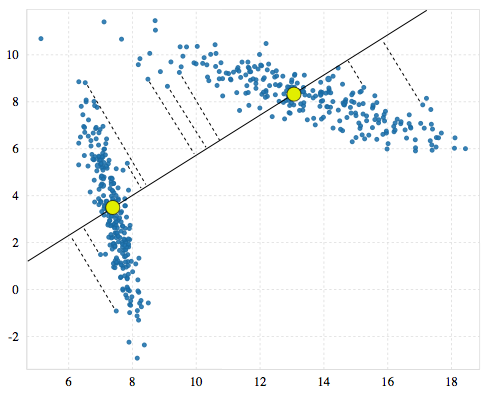
\includegraphics[width=0.7\linewidth]{Grafika/g-means-projection}
\caption{Przykład rzutowania zbioru danych na wektor łączący znalezione środki ciężkości. Źródło: \cite{GMeansExplanation}}
\label{fig:g-means-projection}
\end{figure}

Cały zastosowany algorytm klasteryzacji może być przedstawiony w następujących krokach:
\begin{enumerate}
	\item Jako parametry wejściowe przyjmij zbiór danych oraz ufność testu Andersona-Darlinga.
	\item Wylicz początkowy środek ciężkości: $C = \{\bar{x}\}$.
	\item Wykonaj klasteryzację: C = k-średnich(X, C).
	\item Dla każdej klasy $S_j$ sprawdź jej rozkład testem Andersona-Darlinga:
	\begin{enumerate}
		\item Wylicz dwa środki pochodne $c_j^1, c_j^2$.
		\item Wykonaj ponowną klasteryzację: $\{c^1, c^2\} = k-"srednich(S_j, \{c_j^1, c_j^2\})$.
		\item Wyznacz wektor $u = c^1 - c^2$.
		\item Wyznacz jednowymiarową przestrzeń $S_j '$.
		\item Wylicz wartość statystyki Andersona - Darlinga dla $S_j '$.
		\item Jeśli jest ona większa od wartości krytycznej, podziel klasę $S_j$ na dwie ze środkami $c^1$ oraz $c^2$. Jeśli jest mniejsza, zachowaj poprzedni środek.
	\end{enumerate}
	\item Powtarzaj od kroku 3 dopóki żadne nowe środki nie zostaną dodane.
\end{enumerate}

\subsection{Klasyfikacja}
\quad Aby sklasyfikować powstałe w poprzednim kroku klastry wykorzystano klasyfikator SVM (Support Vector Machine). Problem klasyfikacji wymaga podziału zbioru danych wejściowych na zbiór uczący oraz zbiór testowy. Każdy z elementów zbioru uczącego zawiera wartość oczekiwaną (np. etykieta klasy) oraz jakąś ilość atrybutów (np. wektor cech). Celem SVM jest stworzenie modelu (bazujcego na danych uczących), który przewiduje nieznaną wartość oczekiwaną (etykietę) dla podanego na wejściu elementu zbioru testowego. 

W najprostszej postaci klasyfikator SVM służy do wyznaczenia hiperpłaszczyzny rozdzielającej dwa liniowo separowalne zbiory. Hiperpłaszczyzna ta wyznaczana jest z maksymalnym marginesem, tzn. tak, aby suma jej odległości od najbliższych próbek z obu klas była jak największa (patrz rys. \ref{fig:SVM}).

\begin{figure}[h]
	\centering
	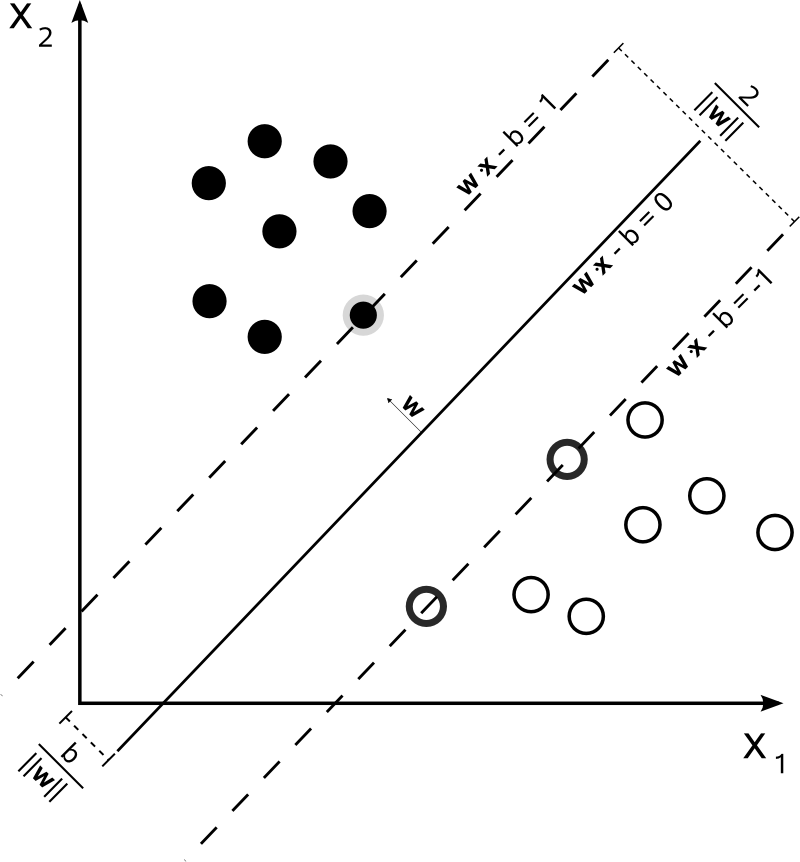
\includegraphics[width=8cm]{Grafika/Svm_max_sep_hyperplane_with_margin}
	\caption{Dwuwymiarowy przypadek hiperpłaszczyzny rozdzielającej dwie klasy z zaznaczonym marginesem. Źródło \cite{SVMWiki}}
	\label{fig:SVM}
\end{figure}

Mając dany zbiór uczący, będący zbirem par składających się z wektora cech oraz etykiety $(x_i, y_i)$, $i = 1,...,l$, gdzie $x_i \in \mathbb{R}^n$ i $y_i \in \{1,-1\}$, maszyna wektorów nośnych (SVM) wymaga rozwiązania następującego problemu optymalizacji \cite{csie}:

\begin{equation}
\label{eq:SVMOptProb}
\min\limits_{w,b,\xi} \frac{1}{2}w^Tw+C\sum_{i=1}^{l}\xi_i
\end{equation}

z ograniczeniem:

\begin{equation}
\label{eq:SVMOptProbCond}
\begin{array}{l}
y_i\left(w^T\phi\left(x_i\right)+b\right) \geqslant 1-\xi_i,\\
\xi_i > 0
\end{array}
\end{equation}


W wielu przypadkach nie można zagwarantować liniowej separowalności zbiorów.  W takich sytuacjach stosuje się tzw. Kernel Trick. Polega to na zwiększeniu wymiaru przestrzeni danych wejściowych, aby w nowej przestrzeni istniała własność liniowej separowalności zbiorów.

W zdefiniowanym wzorami (\ref{eq:SVMOptProb}) oraz (\ref{eq:SVMOptProbCond}) problemie optymalizacji wektor uczacy $x_i$ przekształcany jest do przestrzeni o większym wymiarze dzięki funkcji $\phi$. Parametr $C>0$ jest karą za niespełnienie warunków zadania. Ponadto, funkcja $K(x_i,x_j)=\phi(x_i)^T\phi(x_j)$ jest nazywana funkcją jądra (ang. kernel function). Poniżej wypisano cztery przykładowe funkcje jądra, jakie można spotkać w literaturze poświęconej SVM.

\begin{enumerate}
	\item Liniowa: $K\left(x_i,y_j\right)=x_i^Tx_j$
	\item Wielomianowa: $K\left(x_i,y_j\right)=\left(\gamma x_i^Tx^j+r\right)^d, \gamma > 0$
	\item Radialna funkcja bazwa (RBF): $K\left(x_i,y_j\right)=\exp{\left(-\gamma \|x_i-x_j\|^2\right)}, \gamma > 0$
	\item Sigmoida: $K\left(x_i,y_j\right)=\tanh{\left(\gamma x_i^Tx_j+r\right)}$
\end{enumerate}

W opisywanym module wykorzystana została funkcja RBF (ang. Radial Basis Function).

Aby klasyfikator mógł działać wcześniej należy go wytrenować. Polega to na podaniu mu ciągu wektorów uczących. Opisywany klasyfikator został wytrenowany za pomocą bazy danych MIT-BIH Arrhythmia Database \cite{MITDB}. Gotowy model klasyfikatora wczytywany jest z pliku, w którym zapisane są różne parametry oraz zestaw wektorów nośnych, na których opiera się działanie metody SVM.
